\documentclass[a4paper, 12pt,oneside, english, brazil]{abntex2}

\usepackage{microtype} 			% para melhorias de justificação
% ---
\usepackage{epstopdf}
\usepackage{graphics}
\usepackage{eurosym}

\usepackage[utf8]{inputenc}	
\usepackage[portuges]{babel}
\usepackage{geometry}
\usepackage{amssymb}
\usepackage{hyperref}
\usepackage{color}
\usepackage{float}
\usepackage{setspace}
\usepackage{array}
\usepackage{subcaption}
\usepackage{mathtools}
\usepackage{amsmath}
\usepackage{indentfirst}
\usepackage{graphicx}
\usepackage{multicol,lipsum}
\usepackage[T1]{fontenc}
\usepackage{microtype} 		
\usepackage{epstopdf}
\usepackage{latexsym}
\usepackage{multicol}
\usepackage{multirow}
\usepackage{listings}
\usepackage{listingsutf8}
\usepackage{lmodern}

\begin{document}
\selectlanguage{brazil}
\setlength{\parindent}{1.3cm}
\frenchspacing
%\setlength{\parskip}{0.2cm}

%\maketitle
%%%%%%%%%%%%%%CAPAAAAAAAAAAAAAAAAAAAA%%%%%%%%%%%%%
\begin{capa}
    

	\begin{center}
	
	\begin{figure}[H]
	\centering
	
\includegraphics[width=5cm]{facs.png}
	\end{figure}

		\Huge{Universidade Salvador}\\
		%\large{Departamento}\\ 
		%\large{Programa}\\ 
		\vspace{15pt}
        \vspace{80pt}
        \textbf{\LARGE{Relatório de projeto para acionamento de motor trifásico utilizando um inversor de frequência.}}\\
        \vspace{2pt}
        \large{Acionamento de motor utilizando inversor de frequência em comparação com sua partida direta.}
		%\title{{\large{Título}}}
		\vspace{3,0cm}
	\end{center}

	%\begin{flushleft}
	%	\begin{tabbing}
	%		Aluno: \\
	%		Professor orientador: \\
	%		Professor co-orientador: \\
	%\end{tabbing}
 %\end{flushleft}
%	\vspace{1cm}
	\begin{center}
	  	\large{Dezembro -- 2019}\\
	\large{Salvador -- Bahia}  
	\end{center}
\end{capa}


%%%%%%%%%%%%%%%%%%%%%%%%%%%%%%%%%%%%%%%%%%%%%%%%%%%%%%%%%%%

% % % % % % % % %FOLHA DE ROSTO % % % % % % % % % %

\begin{folhaderosto}
    
	\begin{center}
	
	%\begin{figure}[!ht]
	%\centering
	%\includegraphics[width=2cm]{c:/ufba.jpg}
	%\end{figure}

		\LARGE{Universidade Salvador}\\
		\large{ Faculdade de Engenharia, Arquitetura e Tecnologia da Informação}\\ 
		\large{ Curso de Graduação em Engenharia Elétrica}\\ 
\vspace{15pt}
        
        \vspace{85pt}
        
		\textbf{\LARGE{Relatório de projeto para acionamento de motor trifásico utilizando um inversor de frequência.}}
		%\title{\large{Título}}
	%	\large{Modelo\\
     %   		Validação do modelo clássico}
			
	\end{center}
\vspace{1,5cm}
	
	\begin{flushright}

   \begin{list}{}{
      \setlength{\leftmargin}{6.5cm}
      \setlength{\rightmargin}{0cm}
     \setlength{\labelwidth}{0pt}
     \setlength{\labelsep}{\leftmargin}}

      \item Relatório técnico do esquema e execução de um acionamento de motor trifásico utilizando um inversor de frequência em comparação com uma partida direta de um motor trifásico para projeto da disciplina Acionamentos Elétricos do curso de Engenharia Elétrica da Universidade Salvador.

      \begin{list}{}{
      \setlength{\leftmargin}{0cm}
      \setlength{\rightmargin}{0cm}
      \setlength{\labelwidth}{0pt}
      \setlength{\labelsep}{\leftmargin}}

			\item Alunos: Iuri Fernandes, João Victor Teles, Lucas Menezes, Mariana Sampaio, Naiara Azevedo, Renan Queiroz e Wallace Paixão. \
            \item Professor orientador: Antonia Ferreira Cruz\
      		

      \end{list}
   \end{list}
\end{flushright}
\vspace{1cm}
\begin{center}
		\vspace{\fill}
		 Salvador -- Bahia\\
		 Dezembro -- 2019\\
		 
			\end{center}
\end{folhaderosto}
\newpage
% % % % % % % % % % % % % % % % % % % % % % % % % %
\newpage
\tableofcontents*

\newpage
\listoffigures*

% % % % % % % % % % % % % % % % % % % % % % % % % % %
\newpage
\pagenumbering{arabic}
\chapter{Resumo}

O projeto consiste em acionar a vazio um motor elétrico de indução trifásico utilizando um inversor de frequência para realizar o controle da partida. Assim, pretende-se comparar os efeitos entre o acionamento realizado com o inversor e a partida direta do motor trifásico. Logo, é possível através deste projeto e pelo presente relatório evidenciar na prática a teoria do conteúdo visto em sala de aula.

Para a execução das duas partidas em laboratório foram empregados um conjunto de materiais necessários aos circuitos dos acionamentos previamente esquematizados na teoria. Os equipamentos utilizados foram a Botoeira XB2-EL8325 da SIBRATEC e os elementos fabricados pela WEG, a saber, o Inversor de Frequência CFW080016S2024PSZ, o Motor de Indução de Alto Rendimento Plus, o Relé de Sobrecarga RW27-1D, o Contator CWM9 e o Contator Auxiliar BCXMF01. 


\chapter{Objetivo}

Os objetivos do projeto são:
\begin{itemize}
    \item Acionar o motor elétrico utilizando-se de um inversor de frequência.
    \item Verificar o funcionamento dos inversores de frequência.
    \item Comparar o acionamento em discussão com a partida direta do motor sem a utilização de inversores.
    
\end{itemize}

A finalidade principal do projeto é demonstrar que a utilização de inversores de frequência possibilita aos motores de indução partidas mais suaves, preservando a vida útil dessas máquinas, além de produzir menor impacto na rede ao qual está associado. 


\chapter{Introdução}
O emprego dos equipamentos motrizes para realização de trabalho impulsionou o desenvolvimento humano, tornando viável a execução das mais variadas tarefas que utilizavam tração animal ou semelhante. O avanço em termos desta demanda foi acompanhado pelo surgimento de tecnologias no que diz respeito às máquinas e aos seus recursos de controle.  

Diversas são as categorias dos motores elétricos disponíveis atualmente no mercado, dentre as quais podemos destacar os motores de indução trifásicos, amplamente empregados na indústria. Este destaque para o motor de indução ocorre por conta de sua alta eficiência, baixo custo com manutenção, versatilidade quanto às aplicações e melhores custos-benefícios. Também conhecidos como motores assíncronos, sua construção oferece uma limitação natural quanto ao controle de velocidade e condições de corrente e torque de partida. Tal aspecto limitava o emprego deste motor a aplicações que não demandassem controle de velocidade e altas variações de corrente e torque de partida.

Com o desenvolvimento da eletrônica de potência, a implementação das medidas de controle necessárias para viabilizar o uso irrestrito das máquinas assíncronas foi permitida. Neste ponto destacam-se os Inversores de Frequência como chave eletrônica para partida e controle de motores em corrente alternada. Tendo em vista a importância deste elemento, discutiremos nesse relatório os principais aspectos relacionados a essa tecnologia, seus elementos, os parâmetros elétricos da partida e suas vantagens ou desvantagens com relação à partida direta do motor de indução.  

%escrever sobre o resto de coisas q a gente usou
\chapter{Fundamentação teórica}
Neste capítulo serão tratados os aspectos teóricos dos motores elétricos de indução trifásicos, dos inversores de frequência,

\section{Motor elétrico de indução}

Motores elétricos são as máquinas destinadas a transformar energia elétrica em energia mecânica, geralmente através da interação entre dois campos magnéticos, como no caso do motor de indução. Sendo um dos campos associado aos elementos estacionários da máquina e o outro aos seus elementos móveis. A figura \ref{clas} sugere uma classificação para os motores elétricos:

\begin{figure}[H]
    \centering
    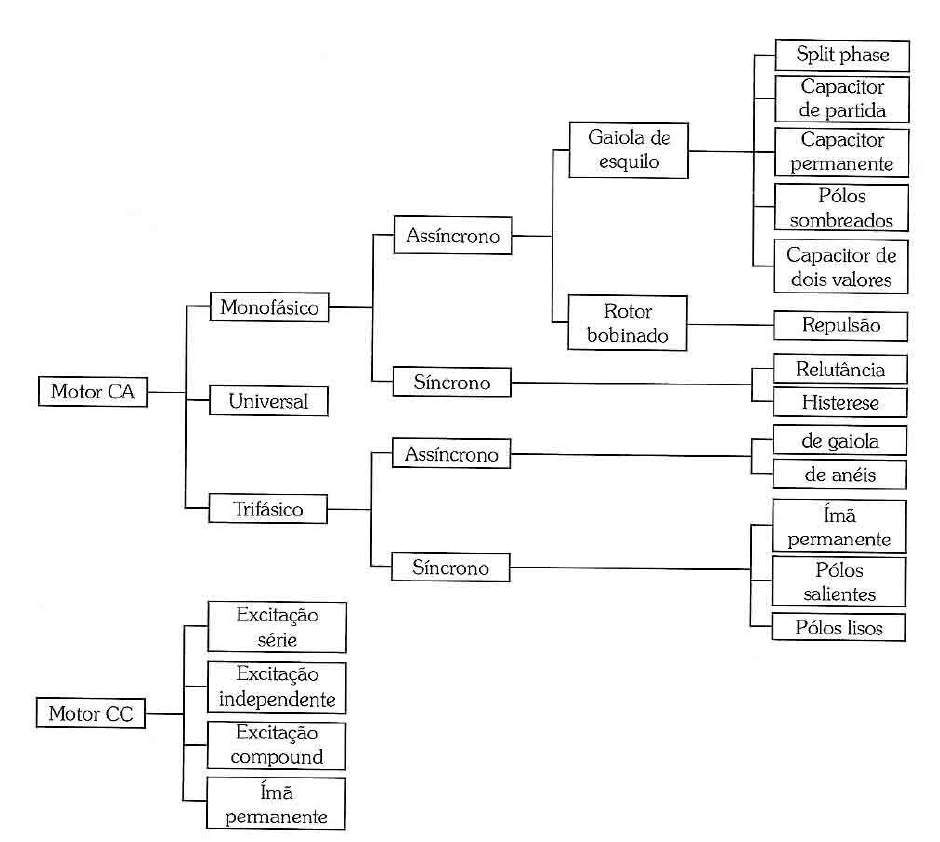
\includegraphics[scale=0.36]{clas.png}
    \caption{Classificação de motores elétricos. Fonte: \protect\shortcite{Franchi}, 2008}
    \label{clas}
\end{figure}

Para o estudo aqui desenvolvido, será adotada a máquina trifásica assíncrona com rotor de gaiola. Esses equipamentos são caracterizados por operarem sempre com rotação inferior à rotação síncrona, daí origina-se a sua denominação habitual.    

A máquina de indução trifásica pode ser dividida em duas partes principais, o estator onde concentram-se as bobinas de armadura, e o rotor. Quando alimentado por uma tensão trifásica, os enrolamentos dos estator fazem surgir no entreferro do motor um campo magnético “girante”, o qual terá uma velocidade de giro conhecida por velocidade síncrona. Esse campo girante é responsável por induzir tensão no circuito do rotor o que, por consequência produz a interação magnética necessária para o funcionamento do motor.

\begin{figure}[H]
    \centering
    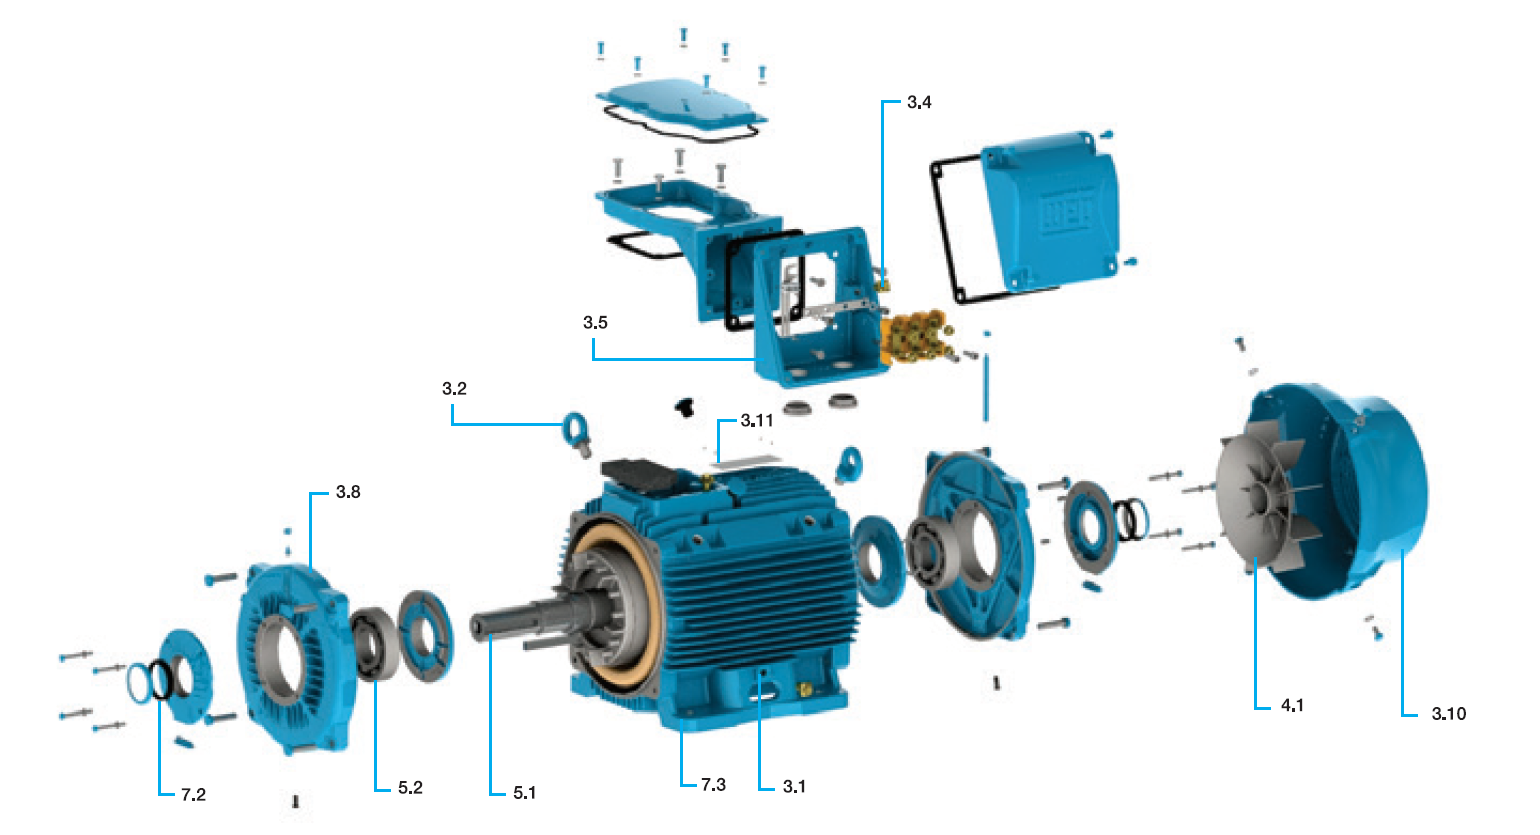
\includegraphics[scale=0.26]{motor.png}
    \caption{Partes de um motor. Fonte: WEGNOLOGY}
    \label{parts}
\end{figure}
%como que poe uma figura com numeros e n poe a legenda????

Os campos girantes do rotor e estator possuem a mesma direção e têm a mesma velocidade, sendo assim são estacionários entre si, no entanto, a velocidade do rotor será sempre inferior à síncrona, o que permite a criação do torque útil no motor elétrico, garantindo existência de corrente induzida no mesmo.

A fórmula matemática que expressa à velocidade síncrona calculada de um motor trifásico é apresentada na equação~\eqref{freq}, sendo $n_{s}$ a velocidade síncrona em rotações por minuto, $f_{e}$ a frequência elétrica de operação em Hz e $p$ o número de polos do motor.

\begin{equation}
    n_{s}=\frac{120 \times f_{e}}{p}
    \label{freq}
\end{equation}

A máquina trifásica está fundamentada em um campo magnético rotativo, que acontece quando um sistema de alimentação trifásica de corrente alternada em polos defasados 120º entre si. A velocidade do motor elétrico trifásico está diretamente ligada ao seu número de polos e à frequência da rede elétrica a qual o motor está sendo alimentado, sendo a quantidade de polos uma característica de fábrica do motor elétrico.

Uma característica importante das máquinas de indução é a relação entre a velocidade síncrona e a velocidade de giro do rotor. A essa relação dá-se o nome de Escorregamento ($s$) expressa pela equação~\eqref{s}, com $n$ equivalente à velocidade do rotor em rotações por minuto.
\begin{equation}
    s=\frac{n_{s}\times n}{n_{s}} 
    \label{s}
\end{equation}

A figura \ref{rot} representa o circuito equivalente ao motor de indução. Da análise desse circuito podemos destacar algumas considerações importantes. A primeira consideração justifica o arranjo propriamente dito, ou seja, o motor de indução trifásico tem representação equivalente à de um transformador e, essa condição impacta em nossos estudos uma vez que as reações no circuito rotórico terão seus efeitos replicados ao estator da máquina. Outra observação importante diz respeito ao efeito do escorregamento sobre o funcionamento da máquina. Fica evidente por observação que o escorregamento produz impacto inversamente proporcional à corrente do rotor e por consequência à corrente de alimentação do motor.

\begin{figure}[H]
    \centering
    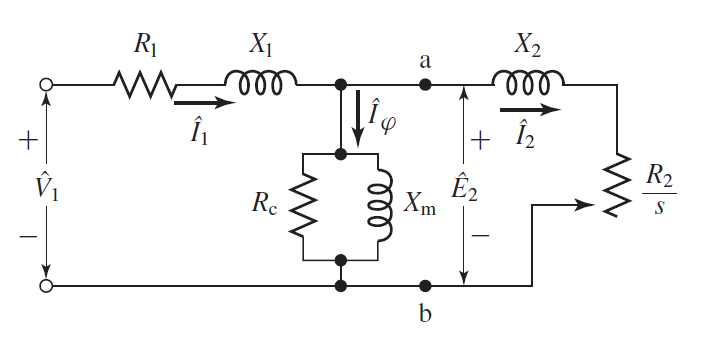
\includegraphics[scale=0.42]{rot.png}
    \caption{Circuito equivalente do motor de indução. Fonte: Fitzgerald and Kingsley, 2014}
    \label{rot}
\end{figure}

Outro aspecto relevante para o entendimento desse relatório é a curva característica da máquina de indução, que pode ser observada na figura \ref{tor}. Da análise dessa curva típica, pode-se concluir que, em operação normal a máquina assíncrona oferece torque variável em razão da rotação sendo que esse tem valor da ordem de 120$\%$ de seu valor nominal na partida, ascende até rotações próximas a 85$\%$ da nominal e então decai para seu valor de operação. 

Essa condição de torque é fruto das interações de cada elemento representativo da máquina e, consequentemente, pode variar de acordo com suas especificações. Para o estudo em questão, as peculiaridades no que diz respeito às diversas curvas típicas não serão objeto de estudo. Cabe destacar aqui que, essa condição de operação tem reflexo no comportamento dinâmico da máquina e por isso não se pode desprezar essas informações na análise.

\begin{figure}[H]
    \centering
    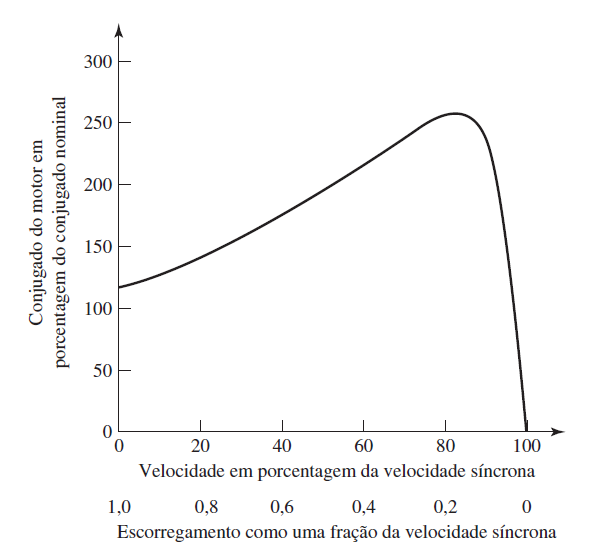
\includegraphics[scale=0.42]{tor.png}
    \caption{Conjugado x velocidade. Fonte: Fitzgerald and Kingsley, 2014}
    \label{tor}
\end{figure}
Ainda com relação à figura \ref{tor} , podemos observar que o valor de conjugado da máquina está diretamente relacionado a velocidade alcançada pelo rotor. Na partida do motor, o conjugado chega em torno de 120$\%$ do nominal para que retirar a máquina da inércia, chegando a atingir seu valor máximo de torque próximo de 250$\%$ do nominal quando o motor atinge por volta de 85$\%$ de sua velocidade síncrona. A partir daí o torque do motor decresce até atingir valor nulo em percentual do nominal quando o motor vai se aproximando da velocidade síncrona.

\section{Chaves de Partida}
As chaves de partida são circuitos por meio dos quais conectamos os motores à rede elétrica. Os elementos constituintes desse circuito têm como função primordial oferecer a proteção necessária para o funcionamento do motor. Adicionalmente, mas não menos importante, as chaves de partida possibilitam adequar a partida do motor às limitações inerentes a rede que o alimenta além de oferecer algum controle nessa condição. Podemos classificar as chaves de partida em dois grupos primordiais, as Chaves de partida convencionais e Chaves de partida eletrônicas.

\subsection{Partida Direta}
A partida direta é um dos tipos de acionamentos de máquinas elétricas onde o motor recebe a alimentação diretamente da fonte de energia trifásica, portanto esse método de partida configura-se em uma das ligações mais simples entre todas as formas de acionamentos de motores.
As principais características da partida direta são:
\begin{itemize}
    \item Conjugado nominal na partida;
    \item Corrente de partida pode chegar a 8 vezes a corrente nominal;
    \item Necessita de dispositivos de acionamento mais robustos;
    \item Custo elevado de manutenção.

\end{itemize}

Devido a partida direta ocorrer com tensão nominal da rede elétrica, aplicada diretamente aos enrolamentos presentes no estator da máquina, é  necessário nesse acionamento alguns dispositivos de proteção, tais como fusíveis e relés de sobrecarga. Sendo os fusíveis dispositivos de proteção contra curtos circuitos e os relés equipamentos programados para a proteção de sobrecargas nos motores elétricos trifásicos. 

\begin{figure}[H]
    \centering
    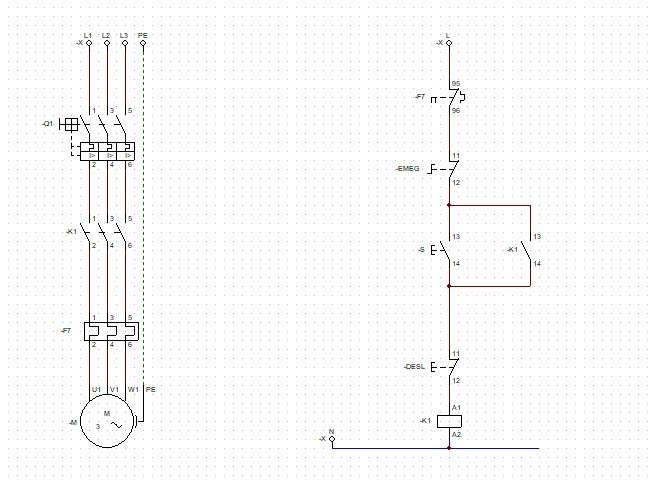
\includegraphics[scale=0.9]{partdir.jpg}
    \caption{Diagrama de comando e de força da partida direta. Fonte: Própria}
    \label{partdir}
\end{figure}

\subsection{Inversor de frequência}

Os inversores de frequência configuram-se como dispositivos capazes de alterar o valor da frequência entregue pela rede no acionamento de outros dispositivos. O princípio de funcionamento dos inversores se baseia em algumas etapas. Primeiramente, o sinal alternado proveniente da rede elétrica é retificado em um sinal contínuo pulsante, através de um circuito de retificação composto por diodos.

Após a passagem pela ponte retificadora o sinal pulsante é filtrado por meio de capacitores em paralelo e uma indutância em série, sendo essa etapa denominada de barramento de corrente contínua. 
Por fim a etapa inversora da operação do processo interno do equipamento consiste em chavear a tensão contínua através de transistores IGBT’s utilizando uma técnica chamada PWM (modulação por largura de pulso). Desta maneira, o sinal DC é convertido novamente em um sinal AC, contudo agora grandezas como frequência e tensão são controladas eletronicamente pelo inversor. 

\begin{figure}[H]
    \centering
    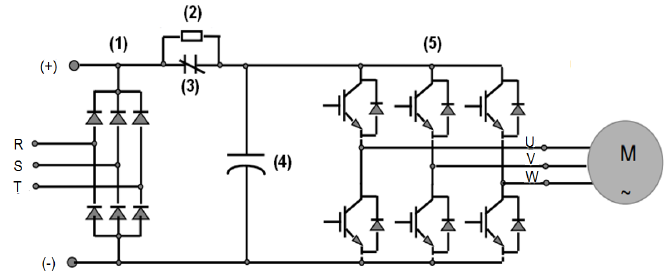
\includegraphics[scale=0.8]{inv.png}
    \caption{Esquema geral de um inversor de frequência. Fonte: Hart, 2011}
    \label{inv}
\end{figure}
Os inversores de frequência podem ser classificados em dois tipos, escalar ou vetorial. 
Basicamente o inversor do tipo escalar é utilizado em aplicações menos robustas como o controle da partida, da parada e a manutenção da velocidade em um valor constante (regulação). Seu funcionamento está baseado no controle da velocidade da máquina através da relação tensão-frequência que graficamente possui uma curva linear como pode ser visto na figura \ref{abaixo}.

\begin{figure}[H]
    \centering
    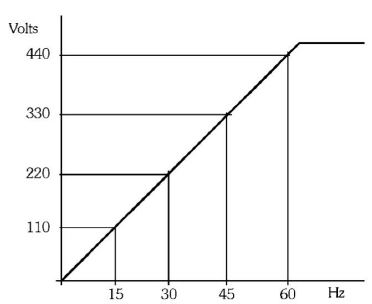
\includegraphics[scale=0.8]{abaixo.png}
    \caption{Gráfico tensão x frequência. Fonte: Franchi, 2014}
    \label{abaixo}
\end{figure}
Já o inversor do tipo vetorial é utilizado em atividades mais complexas, que exigem maior precisão no ajuste de torque e velocidade, onde seu princípio de funcionamento está fundamentado na variação da relação entre tensão e frequência para que assim seja obtido um torque de acordo com a necessidade. 
\subsubsection{CPU (unidade de central de processamento)}
Conhecido como a memória dos inversores de frequência, a CPU é responsável pela concentração de todas as informações, tais como parâmetros e dados do sistema. A CPU pode ser formada por um microprocessador ou um microcontrolador, e é este bloco responsável também pela a formação dos pulsos de disparos para os IGBT’s, por meio de uma lógica de controle específica.

\subsubsection{IHM (Interface homem/máquina)}
Corresponde o meio pelo qual é possível o controlador do inversor parametriza-lo acordo com as suas aplicações requeridas. É possível também neste bloco visualizar o estado de processamento do inversor (através do display).
\subsubsection{Interfaces}
Grande parte dos inversores possui capacidade de ser controlado através de sinais analógicos ou digitais. Assim, por exemplo, quando utilizamos o inversor para controlar a velocidade de giro de um motor AC utilizamos a tensão analógica de comando. Contudo, além da interface analógica, a presença de entradas digitais proporciona a esses dispositivos selecionar através de um parâmetro de programação , por exemplo, qual entrada será considerada válida. 

\begin{figure}[H]
    \centering
    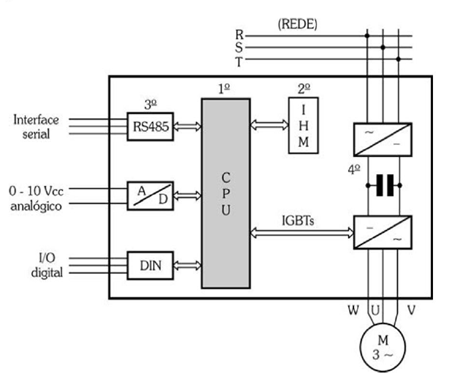
\includegraphics[scale=0.8]{estru.png}
    \caption{Estrutura de um inversor de frequência. Fonte: Franchi, 2014}
    \label{estru}
\end{figure}

\subsubsection{ Etapa de Potência}
Corresponde ao circuito de retificação que alimenta, por meio de um circuito intermediário, denominado de “barramento DC”, o circuito de saída do inversor (módulo IGBT).

\begin{figure}[H]
    \centering
    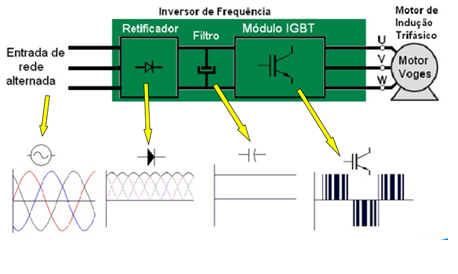
\includegraphics[scale=0.8]{aaa.png}
    \caption{Etapa de potência do inversor.}
    \label{aaa}
\end{figure}

\subsubsection{Partida direta com inversor de frequência}

A principal vantagem do inversor de frequência é poder controlar a velocidade síncrona de motores elétricos. Ao utilizar-se de um inversor de frequência na partida direta de um motor elétrico é possível verificar importantes vantagens para a vida útil da máquina, por exemplo, o inversor de frequência é capaz de reduzir o pico de corrente na partida dos motores. 

Como já dito, nos acionamentos de máquinas elétricas através da partida direta, são verificadas correntes de partidas até oito vezes maior que suas correntes nominais, assim curtos-circuitos, queima de dispositivos de proteção e danificação nos motores são possíveis. Logo, utilizar um inversor de frequência é vantajoso, já que este consegue limitar a corrente de partida em até aproximadamente 1,5 vezes a corrente elétrica nominal.

Portanto, o inversor de frequência é capaz de proporcionar uma partida mais suave em motores, ou seja, utilizando-se desses dispositivos é possível fazer o motor obter sua partida em baixa rotação e ir aumentando sua velocidade gradativamente, prevenindo assim danos mecânicos precoces e aumenta a vida útil do motor.

%pra que merda tem o soft starter aqui??
\subsection{Soft Starter}
O soft starter é um dispositivo eletrônico capaz de limitar a corrente de partida, a fim de tornar a partida e a desenergização de motores mais suave. Esse dispositivo é formado de tiristores SCR’s que são acionados por um circuito elétrico, permitindo assim o controle da tensão eficaz na partida do motor e em seu desacionamento. O valor controlado de tensão aplicado ao motor resultará consequentemente numa corrente limitada, contudo, essa influência restrita à tensão prejudicará o torque resultante da máquina.

\begin{figure}[H]
    \centering
    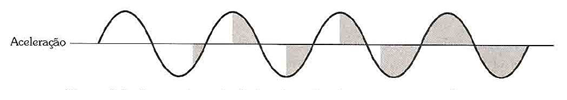
\includegraphics[scale=0.8]{soft.png}
    \caption{Forma de onda aplicada ao motor com Soft starter. Fonte: Franchi, 2014}
    \label{SOFT}
\end{figure}

O gráfico \ref{xx} demonstra o efeito direto da ação do Soft Starter aplicado à limitação da corrente de partida de motores. Fica evidente aí que tal qual outras chaves pautadas na manipulação de tensão no terminal do motor, o Soft Starter é eficiente se o objetivo for, restritamente, limitar os efeitos de corrente na partida da máquina.

\begin{figure}[H]
    \centering
    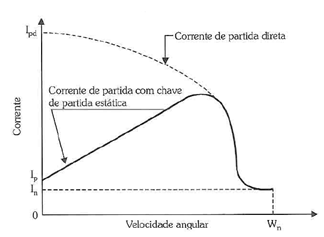
\includegraphics[scale=0.8]{graf.png}
    \caption{Corrente X Tempo - Motor com Soft starter. Fonte: Franchi, 2014}
    \label{xx}
\end{figure}

\subsection{Diferença entre soft starter e inversores de frequência }
O soft starter é um dispositivo capaz de atuar em vários motores, função denominada de By-pass, contudo esses não são capazes de controlar a velocidade, sendo habilitados para atuar apenas na partida e/ou desenergização dos motores.

Já os inversores de frequência, ao contrário do soft starter, são capazes de controlar apenas um motor por vez, contudo o inversor além de controlar a partida do motor é habilitado a alterar a velocidade de giro da máquina de forma que o seu torque permaneça em um valor adequado. Ademais, o inversor é usado também para proteção contra falta de fase e/ou sobrecarga, é ainda programado para atuar na frenagem, na monitoração da frequência máxima/mínima e da corrente elétrica, além de proteger o motor através da determinação da corrente nominal. 
\section{Botoeiras e Contatores}
As botoeiras são dispositivos de comando com a função de estabelecer ou interromper a carga em um circuito de comando, a partir de um acionamento manual. Os tipos de botoeira variam quanto as cores, formatos e aplicações, no caso deste projeto utilizamos botoeiras duplas. 

\begin{figure}[H]
    \centering
    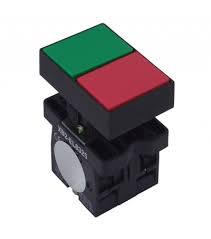
\includegraphics[scale=0.45]{botoeira.jpg}
    \caption{Botoeira dupla.
. Fonte: SIBRATECX}
    \label{botr}
\end{figure}

Seu padrão de classificação de cores segue a seguinte lógica:
Para ligar, dar partida ou arranque a cor será preta, para desligar ou parar teremos a cor vermelha, para eliminar uma condição perigosa ou iniciar um retorno a cor será amarela e outras funções não específicas ela pode ser azul ou branca.

Os contatores são dispositivos eletromecânicos que permitem o acionamento de cargas que exigem correntes maiores, como em nosso caso, os motores trifásicos. Sua estrutura é composta de uma bobina, um núcleo e um conjunto de contatos de força e de comando. Seu funcionamento é baseado em fenômenos magnéticos responsáveis pelos ligamentos ou desligamentos dos contatos.

\begin{figure}[H]
    \centering
    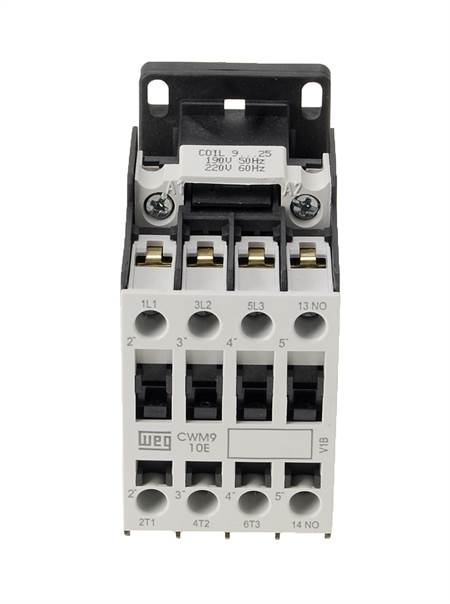
\includegraphics[scale=1.2]{contator.jpg}
    \caption{Contator CWF09. Fonte: WEG}
    \label{cont}
\end{figure}
Os tipos de contatos se resumem a normalmente abertos (NA) e normalmente fechados. Os primeiros permanecem sempre na posição aberta, e se fecham quando acionados, permitindo passagem de corrente elétrica, enquanto os segundos permanecem sempre na posição fechada, e se abrem quando acionados, interrompendo a passagem de corrente elétrica. Além disso temos os contatos comutadores, os quais possuem as duas funções no mesmo contato, com uma parte NA e outra NF e são empregados para comutar entre diferentes partes de um circuito.

Ainda são divididos em contatos de força, utilizados para manobrar os circuitos de força, cargas resistivas ou indutivas e contatos auxiliares, empregados para manobrar os circuitos de comando, intertravamento e sinalização, não devendo ser utilizados para manobrar cargas em substituição aos contatores de força.

\section{Relé de Sobrecarga}
Empregados para garantir a integridade de um equipamento ou processo elétrico, os relés de sobrecarga são dispositivos de proteção responsáveis por proteger os motores elétricos de possíveis anomalias, sendo a mais comum o sobreaquecimento do motor elétrico. 

\begin{figure}[H]
    \centering
    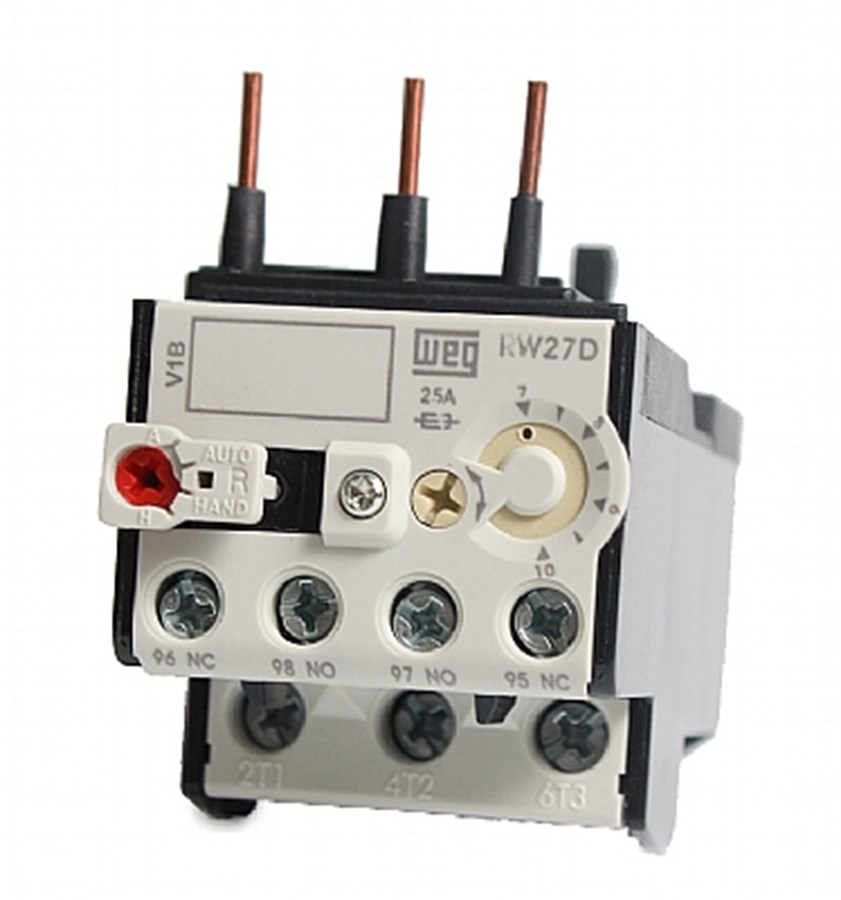
\includegraphics[scale=0.3]{RW17weg.jpg}
    \caption{Relé de sobrecarga RW17D. Fonte: WEG}
    \label{reeet}
\end{figure}

Ao trabalhar com especificações que não se enquadram ao motor elétrico utilizado, danos podem ocorrer em suas bobinas provocando aquecimentos e defeitos em sua estrutura de isolação, podendo gerar curto-circuitos. Assim, neste momento de sobreaquecimento,o relé entra em ação. Suas lâminas bimetálicas de diferentes coeficientes de temperatura aquecem e deformam as laminas, fazendo com que ativem o relé, desarmando o circuito do motor, como também o circuito de comando através de seus contatos auxiliares.
Desta forma o motor só poderá ser ligado quando ocorrer uma ação manual de rearme.

\chapter{Materiais e Métodos do Projeto de Acionamento}
Para o estudo proposto, empregaremos um motor de indução trifásico modelo W22 WEG, Linha alto rendimento Plus operando sem carga axial, alimentado com tensão 220V, 60 hertz. Para fins comparativos, serão realizados acionamentos da unidade motriz através de partida direta e posteriormente controlada por um DRIVE CFW-08 da WEG. O diagrama de partida do motor com inversor de frequência pode ser visto na figura \ref{esquema}, confeccionado através do software CADeSIMU.

\begin{figure}[H]
    \centering
    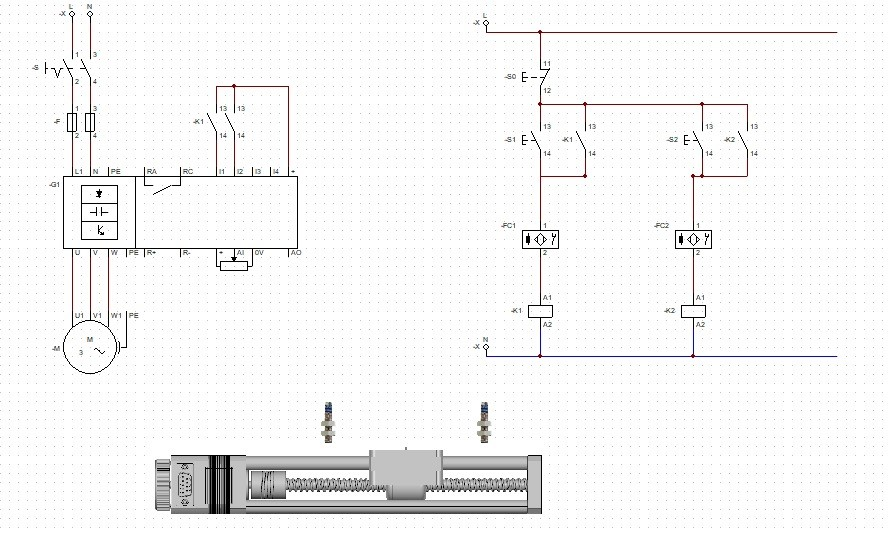
\includegraphics[scale=0.6]{esquema.jpg}
    \caption{Diagrama de Comando e Força para Partida com Inversor
. Fonte: Própria}
    \label{esquema}
\end{figure}
O projeto considerará as condições nominais de operação da máquina, sendo apontado para ambos os casos o conjunto dos equipamentos destinados à Comando, Controle e Proteção. Os itens destinados à montagem final devem atender, concomitantemente à critérios técnicos e a sua disponibilidade.

\section{Carga Motriz}
Foi utilizado um motor elétrico trifásico de 0.25cv de potência, 1705 RPM e 4 polos, que será conectado a uma rede de alimentação trifásica de 220Vac/60Hz. A corrente nominal informada pelo fabricante é de 1,03A e possui como fator de corrente de partida: Ip/In=4,7, além de trabalhar em regime S1 com rotor gaiola de esquilo.
\begin{figure}[H]
    \centering
    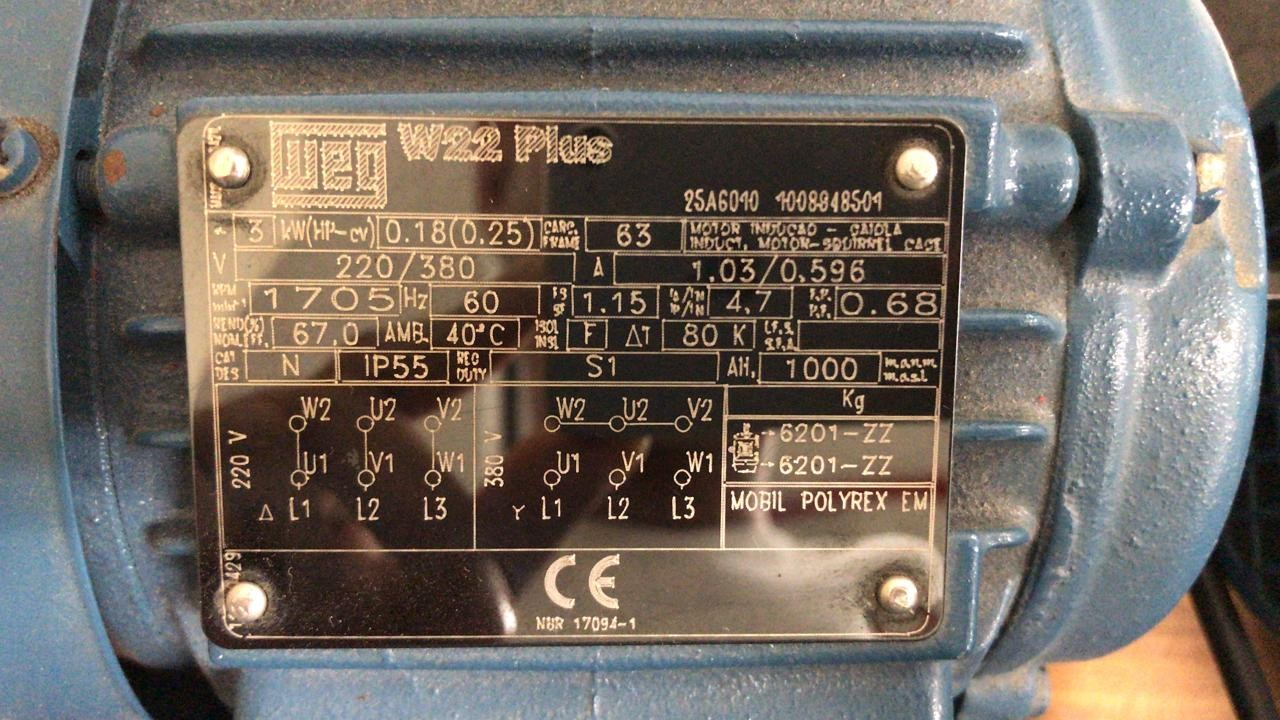
\includegraphics[scale=0.45]{motor.jpg}
    \caption{Dados de placa do motor utilizado.
. Fonte: Própria}
    \label{motooor}
\end{figure}

\begin{figure}[H]
    \centering
    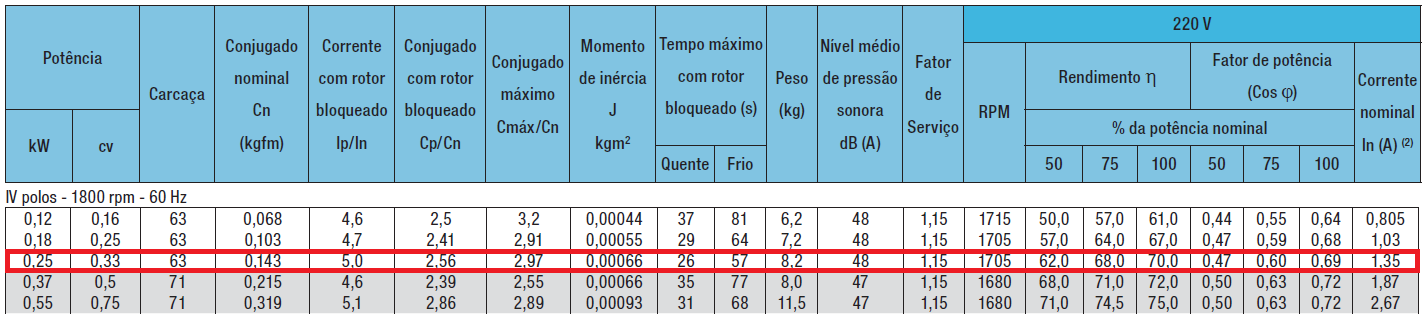
\includegraphics[scale=0.45]{tabelinhaaa.png}
    \caption{Características e parâmetros elétricos variados de um motor. Destacado com o retangulo vermelho temos os parâmetros do motor utilizado.
. Fonte: Manual Motores de Indução WEG}
    \label{tab}
\end{figure}
\newpage

\section{Lista de materiais e equipamentos}

Foram utilizados diversos materiais eletro-eletrônicos para a prática dos projetos. Tais utensílios estão identificados na tabela \ref{uten}, com exceção dos cabos de conexão utilizados rotineiramente em construção de circuitos e oferecidos pelo laboratório. Para a partida direta utilizou-se os contatores, relé de sobrecarga e botoeira. Enquanto que a partida com o inversor , objeto de estudo do nosso trabalho, utilizou-se apenas o relé de sobrecarga (apesar das condições de operação da bancada permitir apenas o uso de um simples disjuntor) e o inversor de frequência.

\begin{table}[H]
\centering
\begin{tabular}{|l|l|l|}
\hline
Equipamento     & Fabricante  & Modelo \\\hline
Inversor de frequência & WEG & CFW080016S2024PSZ \\\hline
Motor de Indução & WEG & ALTO RENDIMENTO PLUS \\\hline
Relé de Sobrecarga & WEG & RW27-1D \\\hline
Contator & WEG & CWM9 \\\hline
Contato auxiliar & WEG & BCXMF01  \\\hline 
Botoeira 1NA + 1NF &SIBRATEC & XB2-EL8325 \\\hline
\end{tabular}
\caption{ Elementos utilizados na prática em laboratório. }
\label{uten}
\end{table}

 
\section{Procedimentos}
Nesta seção serão apresentados os procedimentos realizados para a execução do acionamento do motor através do inversor de frequência.

\subsection{Dimensionamento do Inversor de Frequência}
Com a informações obtidas do motor consultamos o catálogo do fabricante, a disponibilidade do material no laboratório e escolhemos um inversor que atendeu as seguintes características requeridas.

\begin{itemize}
    \item Tensão de entrada: 220 V
    \item Corrente nominal: 1,03 A
    \item Potência nominal: 0,18 KW
\end{itemize}

Todos os demais parâmetros e funções são de caráter opcional. Assim, os dados nominais de corrente, tensão e potência do inversor de frequência, como pode ser visto na figura \ref{cat}, são aproximadamente equivalentes ao nominal do motor. 
Apesar de já ter um catálogo tabelado que facilita o dimensionamento do inversor podemos calculá-lo segundo \shortciteN{franchi} através da equação ~\eqref{dim}. Assim otemos o valor de corrente do inversor, onde V é a tensão da rede em volts, P é a potência nominal do motor em Watts e $\phi$ é o fator de potência do inversor, comumente igual a 0.8.
\begin{equation}
C_{I}=\frac{P}{V \times \phi}= \frac{180}{220 \times 0.8}= 1.026 A
    \label{dim}
\end{equation}

Para iniciar o processo é necessário primeiramente parametrizar o inversor para exercer a função desejada de maneira especificada, por exemplo, se o inversor funcionará como escalar ou vetorial. Os parâmetros podem ser observados na tabela \ref{param}.

\begin{figure}[H]
    \centering
    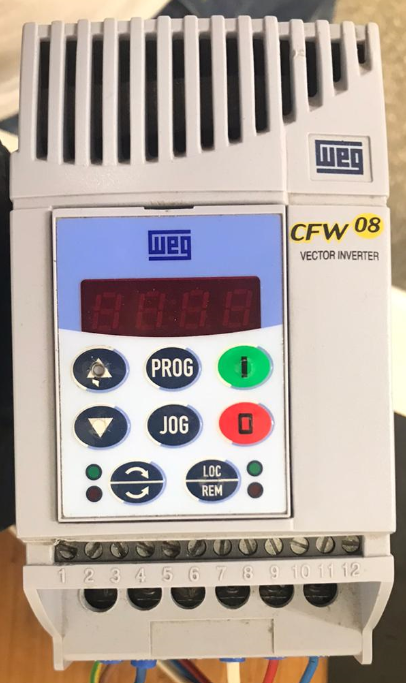
\includegraphics[scale=0.6]{inver.png}
    \caption{Inversor de Frequência utilizado no projeto.
. Fonte: Própria}
    \label{inver}
\end{figure}


\begin{figure}[H]
    \centering
    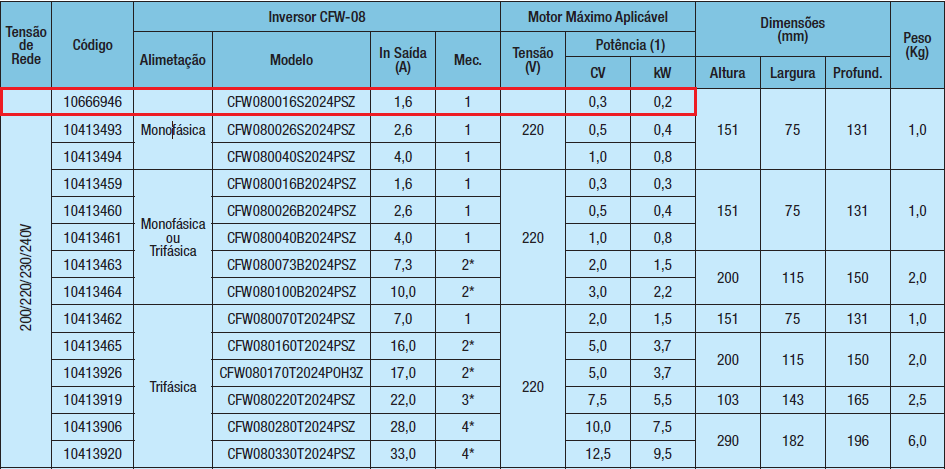
\includegraphics[scale=0.5]{catalogo.png}
    \caption{Parte do catálogo do fabricante com a sinalização do dispositivo escolhido. Fonte: Manual do Inversor de frequência WEG}
    \label{cat}
\end{figure}

\begin{table}[H]
\centering
%\resizebox{0.5\textwidth}{!}{\textwidth}
\begin{tabular}{||lp{2.0cm}||lp{2.0cm}||lp{4.0cm}||lp{6.0cm}||}
\hline
Passo &	Parâmetro	& Função	& Valor \\\hline 
1	& P000	& Parâmetro de acesso	& 5 \\\hline
2	& P204	& Restaurar parâmetros de fábrica	& 5 \\\hline
3 & P000	& Parâmetro de acesso	& 5 \\\hline
4 & P202	& Modo escalar/ vetorial	& 0=Escalar linear/ 1=Escalar quadrático/ 2=Vetorial \\\hline
8	& P156 &	Fator de serviço do motor &	1,15 \\\hline
9	& P133	& Frequência mínima 	& 0 \\\hline
10	& P134	& Frequência máxima	& 60 \\\hline
11	& P100	& Tempo de aceleração	& 10 \\\hline
12	& P101	& Tempo de desaceleração & 	9 \\\hline
13	& P220	& Seleção da fonte; Local/Remoto	& 0 \\\hline
14	& P221	 & Seleção da referência de velocidade &	0 \\\hline
15	& P231	& Seleção do sentido de giro &	2 \\\hline
16 &	P229 &	Seleção de comandos	& 0 \\\hline
\end{tabular}

\caption{ Parametrização inversor de frequência. }
\label{param}
\end{table}

\subsection{Dimensionamento do Relé de Sobrecarga}
A sobrecarga é caracterizada como a elevação da corrente elétrica acima dos valores nominais, mas inferior à verificada numa situação de curto circuito. Este tipo de situação em regime permanente leva a deterioração dos componentes de uma instalação.
É função do relé de sobrecarga proteger a integridade desses componentes, seu funcionamento se baseia em contatos bi metálicos que se dilatam em temperaturas distintas e interrompem o circuito.  
A figura \ref{rele} mostra as características do relé de sobrecarga escolhido. 

\begin{figure}[H]
    \centering
    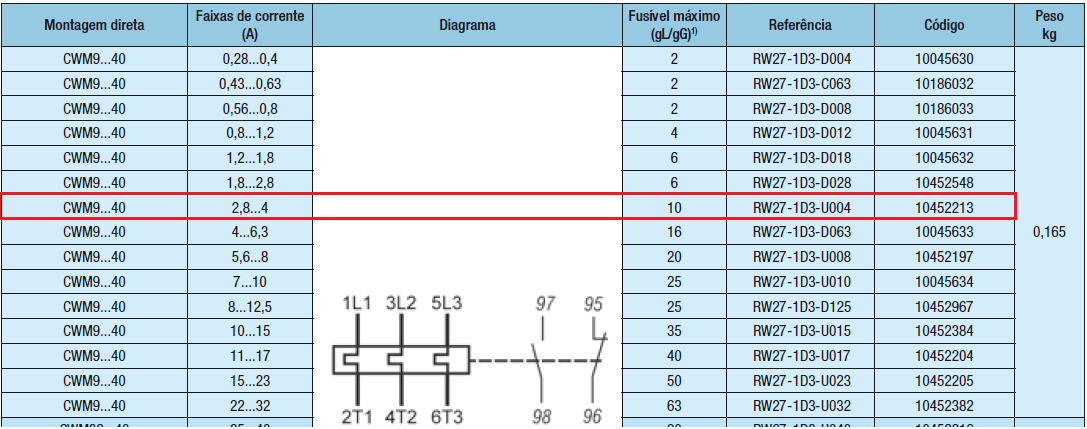
\includegraphics[scale=0.5]{rele.png}
    \caption{Parte do catálogo do fabricante com a sinalização do dispositivo escolhido. Fonte: Manual da WEG}
    \label{rele}
\end{figure}

\chapter{Resultados e Discussões}


Após a montagem de toda estrutura, tanto de alimentação do motor, quanto de sua proteção e a parametrização do inversor de frequência, foi possível como previsto dar inicio a partida do motor dentro de uma faixa de frequência determinada na parametrização, sendo o valor escolhido o de 60 Hz, assim como o tempo de aceleração adotando-se dez segundos. Por motivos de funcionamento do inversor, utilizou-se o modelo escalar e com o auxilio do amperímetro e do multímetro foi possível fazer as análises necessárias de corrente e tensão. Foi feito também o acionamento do motor através da partida direta, para que fossem realizadas algumas comparações.

Durante o acionamento do motor com a utilização do inversor a corrente de pico máxima encontrada foi de 0,93 A e a corrente média alcançou o valor de 0,376 A, enquanto na partida direta a corrente de pico atingiu o valor de 0,96 A e um valor médio de 0,588 A .

\begin{figure}[H]
    \centering
    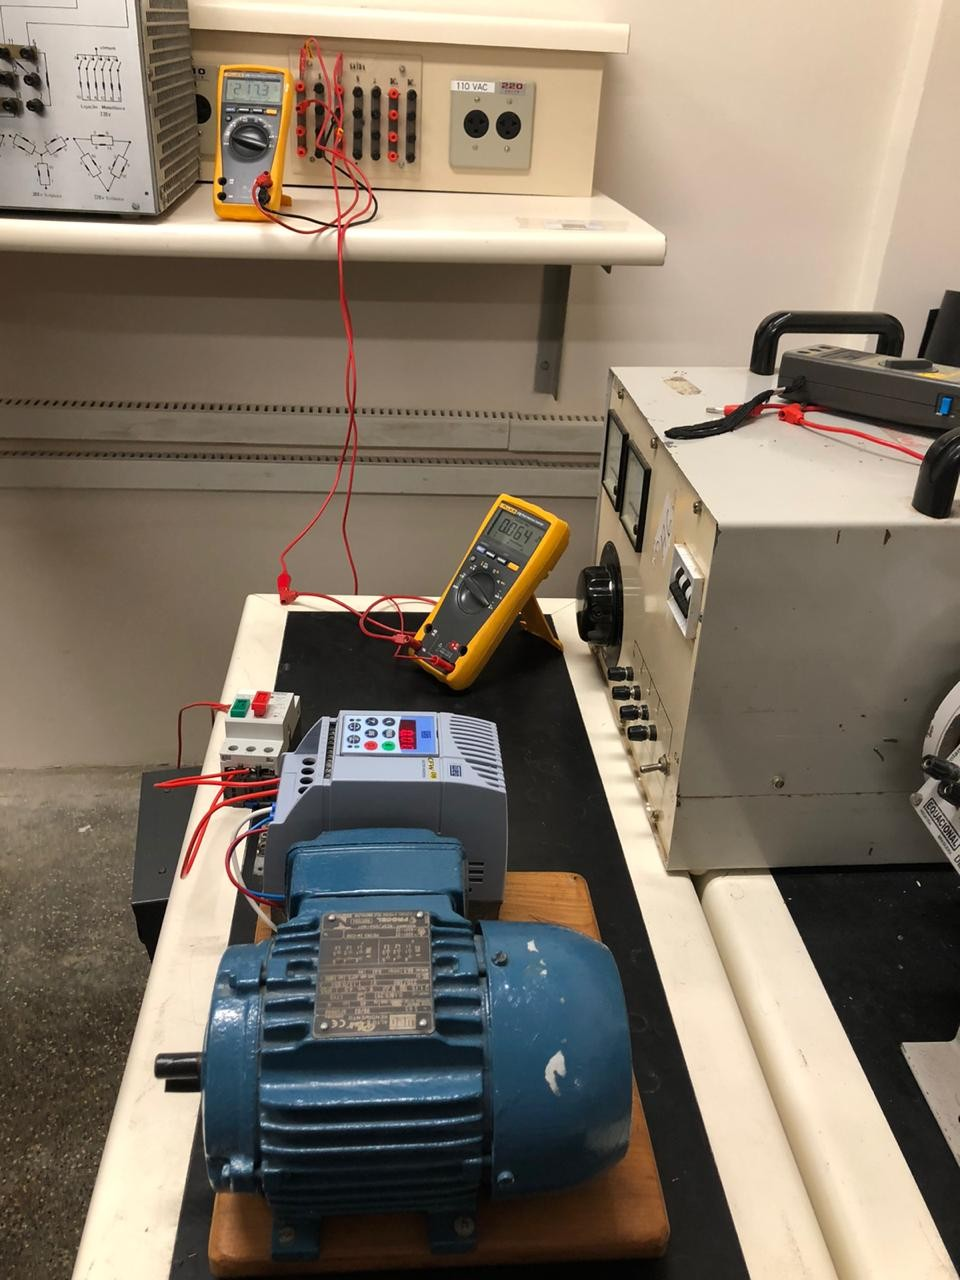
\includegraphics[scale=0.26]{partidinha.jpg}
    \caption{Modelo de partida com o inversor de frequência. Fonte: Própria}
    \label{partid}
\end{figure}

\begin{figure}[H]
    \centering
    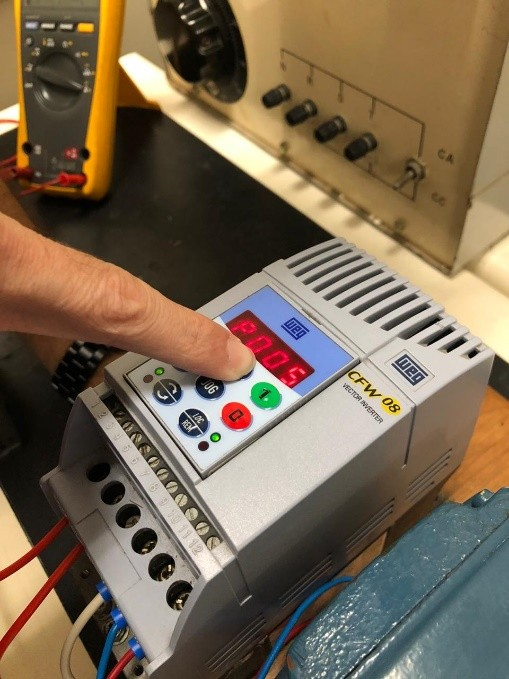
\includegraphics[scale=1.0]{parametr.jpg}
    \caption{Parametrização do inversor. Fonte: Própria}
    \label{haha}
\end{figure}

\begin{figure}[H]
    \centering
    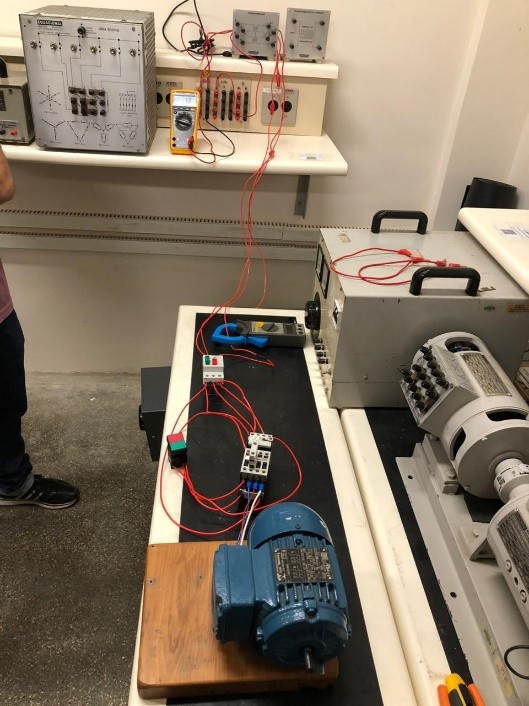
\includegraphics[scale=1.0]{partidadireta.jpg}
    \caption{Modelo de partida direta sem o uso do inversor. Fonte: Própria}
    \label{direct}
\end{figure}

Embora os valores de corrente de pico experimentais sejam pequenos ,já que estamos trabalhando com motores a vazio, percebe-se que a corrente de partida realmente diminui na partida com o inversor de frequência como visto na teoria. Assim o funcionamento deste artifício é testado, comprovado e nos permitiu ainda visualizar uma gama de facilidades oferecidas por ele. Testamos o controle de rampa de aceleração do inversor com 10 e 20 segundos e ainda variados ranges de frequência de alcance do inversor.  


\chapter{Conclusões}
Os propósitos principais do projeto foram atestar as diversas vantagens do inversor de frequência e comparar a sua partida com uma simples partida direta através de acionamentos elétricos. Dentre estes diversos benefícios da utilização do inversor de frequência a melhora no desempenho da máquina e sua suavização e redução do pico de corrente na partida do motor foram os mais significativos percebidos em laboratório. Ainda foi possível observar a redução da corrente média de operação, corroborando para um consumo de energia reduzido com a mesma eficiência.

Embora a prática necessite ser mais robusta e longa para que possamos observar mais vantagens da partida com o inversor de frequência, outras vantaens são relacionadas a ele como:
\begin{itemize}
    \item Redução do nível de ruído dos sistemas.
    \item Excelente regulação de pressão e vazão, em caso de bombas ou compressores.
    \item Economia de energia elétrica .
    \item Controle simplificado de motores elétricos.
    \end{itemize}
    
Agora comparando com o soft starter, o inversor permite fazer não só o controle de tensão mas também da frequência, o que aumenta as possibilidades de controle dos parâmetros de acionamentos, permitindo assim um ajuste mais fino e preciso, assim concluimos que a utilização do Inversor de frequência para o acionamento de um motor elétrico trifásico é uma das melhores opções possíveis apresentada na teoria e evidenciadas na prática.

\chapter{Referências Bibliográficas}
\footnotesize{

\noindent FRANCHI, Claiton Moro. Acionamentos elétricos. Editora Saraiva, 2018.\\

\noindent UMANS, Stephen D. Máquinas Elétricas de Fitzgerald e Kingsley-7. AMGH Editora, 2014.\\

\noindent HART, Daniel W. Power electronics. Tata McGraw-Hill Education, 2011.\\

\noindent WEG, W. M. Inversor de Frequência. manual do usuário CFW-08, 2012. 2016.\\

\noindent FRANCHI, Claiton Moro. Inversores de frequência: teoria e aplicações. Saraiva Educação SA, 2009.\\

}


\end{document}



